\section{Improved Hyperparameter Tuning} \label{sec-hyperparam-optimization}
% Tilmann: this seems very different from the other optimizations. More like a tool. 
Hyperparameters of a machine learning model greatly impact the quality of the model.
There are three common techniques for tuning the hyperparameters, namely, grid search, random search, and Bayesian hyperparameter search \cite{hutter2011sequential,snoek2012practical}.
In this section, we propose three techniques to improve the process of hyperparameter tuning.

\subsection{Search unpacking}
Existing machine learning libraries provide black-box operations for performing hyperparameter tuning.
However, the search process consists of multiple training operations that only differ in hyperparameters.
Therefore, instead of using black-box operations, we consider each training run in the hyperparameter tuning process as a separate operation.
This enables us to apply both the reuse and warmstarting operations to individual training operations in hyperparameter tuning.
%To optimize the grid and random search operation, we first transform them into several model training operations through a simple process called grid unpacking.
%In grid unpacking, each training operation is considered a separate workload.
%Figure \ref{fig-grid-unpacking} shows an example of grid unpacking for a simple SVM Model which has the two hyperparameters penalty (C) and learning rate.
%After unpacking, the reuse optimizations techniques discussed in Section \ref{sec-reuse-and-warmstarting} can be applied.
%\begin{figure}
%\centering
%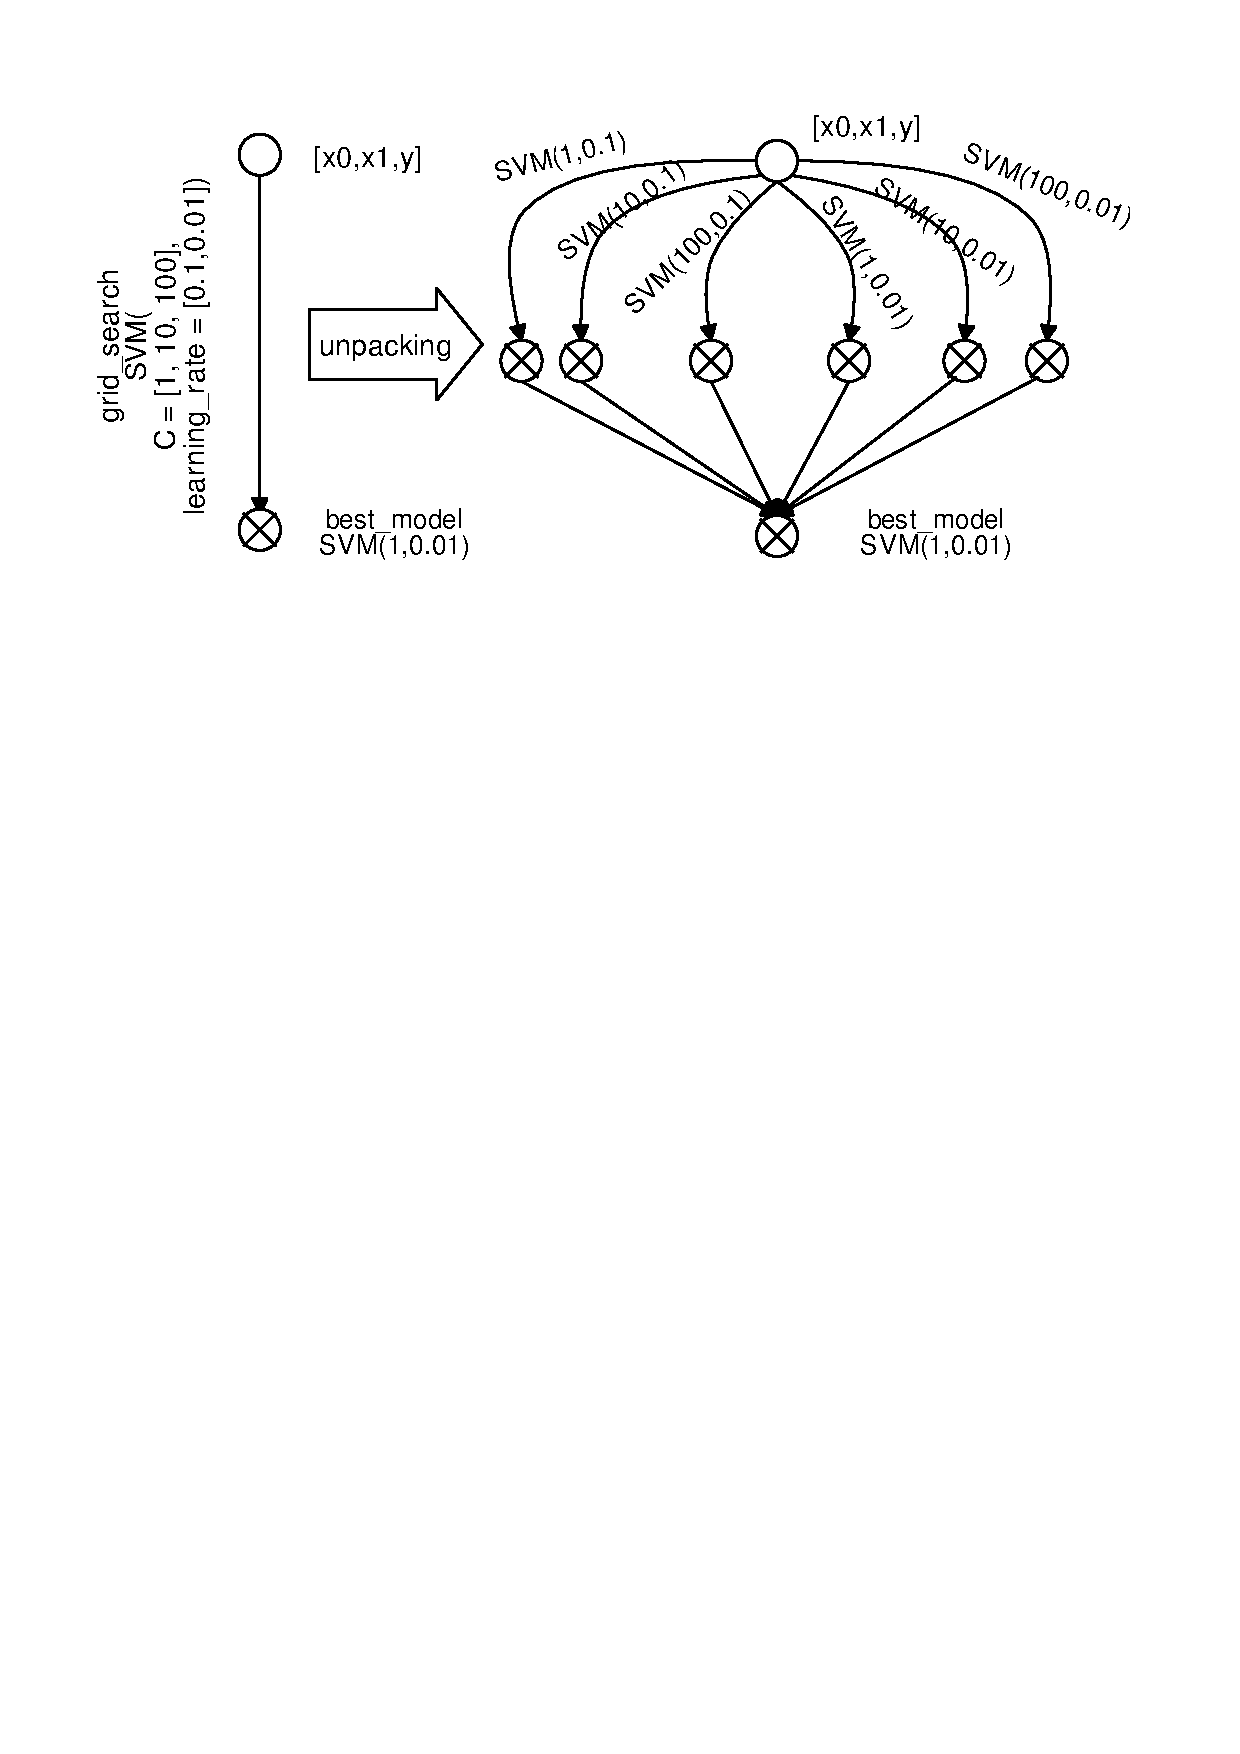
\includegraphics[width=\columnwidth]{../images/grid-unpacking}
%\caption{Result of unpacking on a small grid for SVM model. The hyperparameters are C=[1, 10, 100] and learning rate=[0.1, 0.01]}
%\label{fig-grid-unpacking}
%\end{figure}

\subsection{Automatic Search Space Definition}\label{sub-section-automatic-search-definition}
A major challenge in all the hyperparameter tuning techniques is defining the appropriate search space.
For every hyperparameter, the search space is defined as a probability density function, where values are drawn randomly according to the probability distribution.
Currently, the probability density functions are defined through trial-and-error.
Therefore, users may need to re-execute a hyperparameter tuning operation multiple times with different search spaces to achieve good results.
Novice users, especially, suffer from this problem, as they typically lack the knowledge to define a proper search space.

Using the experiment database, we can propose search space to the users.
For every model group in the experiment database, we proceed as follows.
First, we extract all the hyperparameter values for the model group.
Then, we estimate the distribution of every hyperparameter using density estimation methods.
\todo[inline]{I think a simple Histogram estimation should suffice here. I need to run some quick experiments to Histogram vs Kernel density estimation.}
When a user executes a hyperparameter search in their workloads, we propose the estimated distributions as search space to the user.

One drawback of this approach is that a model group should have enough models with different hyperparameters, in order for the density estimation method to accurately estimate the probability distribution for the hyperparameters \cite{silverman2018density}.
As a result, we can only propose a search space, when there are enough models inside a model group.
In the experiment section, we evaluate the effect of the number of available hyperparameter values on the estimated distribution.
\todo[inline]{I still need to figure out how to design a meaningful experiment for Automatic Search Space definition, since there is no baseline that we can compare ourselves with.
One approach would be to perform multiple hyperparameter tunings with very large budgets in a much bigger search space than the one recommended by our method. We then check how many times the best model found by the search falls in the search space that we defined. }

\todo[inline]{We can also prune the search space by removing the regions that do not yield in good quality models. Since for every hyperparameter value in the experiment database, we have know the resulting model quality, we can only estimate the density for the hyperparameter values that result in a model quality greater than a threshold.}


%\subsubsection{Explorer unit}
%One problem when defining the search space having few instances for some specific hyperparameters.
%To address this issue, we design a component called the explorer unit.
%After a workload is executed, we first determine if there are similar workloads in the experiment database.
%Similar workloads are defined workloads that operate on the same dataset.
%In case the number of the similar workloads is below a threshold, we invoke the explorer unit to automatically propose values for hyperparameters and find the performance of the model trained using each hyperparameter setting.
%%\todo[inline]{This can be defined as a combination of the existing 'best-practices' and a random walk}

\subsection{Fast Bayesian Hyperparameter Tuning}
One drawback of the Bayesian hyperparameter tuning is that it requires many initial random trials until it starts to propose promising hyperparameters \cite{hutter2011sequential,snoek2012practical}.
By utilizing the experiment database, we devise a strategy to decrease the number of initial trials (or in some cases avoid it altogether).
As a result, when users perform bayesian hyperparameter tuning in their workload, they receive promising hyperparameters faster.

Our solution is as follows.
For every existing model group in the experiment database, we start a Bayesian tuning process.
A model group is a set of models that only differ in their hyperparameter values.
We then initialize the search process by including the existing hyperparameters and the corresponding model quality from the model group.

When users submit a workload, there are two possible scenarios.
In the first scenario, the user defines a model training operation in the workload but does not specify any hyperparameters and requests promising hyperparameter values.
In this case, we first find the model group that this workload belongs to.
Then, from the corresponding Bayesian tuning process, we get the proposed hyperparameters to train the model.
In the second scenario, a user may specify a Bayesian hyperparameter tuning process with a specific budget inside their workload (we call this a user-defined Bayesian hyperparameter tuning).
In this scenario, similar to the first scenario, we find the corresponding Bayesian tuning process and utilize it as a starting point for the user-defined Bayesian hyperparameter tuning process.
As a result, the user-defined Bayesian hyperparameter tuning immediately starts to propose promising hyperparameters as it does not need to perform the initial random trials.

%Next, we plan to extend the Bayesian hyperparameter search to the entire pipeline, typically referred to as AutoML \cite{thornton2013auto}.
%In AutoML, the decision to perform an operation on the training dataset is also considered a hyperparameter.
%As a result, we can propose a promising machine learning \textit{pipelines} instead of just hyperparameters for the model.

%\subsubsection{Avoiding Local Optima}
%\todo[inline]{This may not be a problem though. I can find out more after running some more experiments.}
%Warm starting for hyperparameter optimization and AutoML have the benefit of reducing the overhead of computing many trials.
%However, inserting the data from the experiment database into the optimization process may lead the search into local optima.
%This could decrease the chance of finding the best hyperparameter setting.
%However, our automatic search space definition mechanism alleviates this problem as it explores the regions beyond what is currently defined in the experiment database.
%Furthermore, we propose a simple \textit{adaptive warmstarting} method that chooses promising points.